%!TEX root = ../main.tex

% 1000-2000 Words
% 
% Merge with evalutation


\chapter{Implementation and Evaluation}

For clarity, we present the implementation and evaluation together and split the presentation by the natural split in the code which is the server and application.

\section{Application}
\subsubsection{Android}
Android has been chosen for this application due to the large success and market hold of the operating system.

Primarily I will be targeting to support Android versions down to API level 16 (Jelly Bean 4.1).
This decision has been made as figure \ref{fig:AndroidVersions} shows that by supporting this far back, my application will be compatible with over 95\% of current phones. 
Older versions than this will not be targeted, as development and testing time is limited and many features will have to be limited due to lacking functionality within these older versions.

\subsubsection{Material Design}
In order to keep up with a modern and usable design for KidQuest, I have chosen to adhere to the most current standards set by Google for material design.

\subsubsection{Google Cloud Messaging}
The app will be responsible for relaying information between the parent and child clients in a reliable and timely manner.

\subsection{Facebook SDK}
In order to achieve better functionality in the social media features within the app, I will need to gather access to certain information about the user with their strict and explicit permission. 
Tying in the Facebook SDK into the app is the easiest way to gather this information in a secure manner that does not supersede the users wishes.
For example, using the Facebook SDK, I can prompt the user to allow the app permission to gather the users friends list, detect which of them also have used the app and have connected it to facebook and connect the two users as friends within my app.
%TODO: Reword this shit
This technology has strict ethical concerns however, as gathering this information on children has a potential risk for privacy and security concerns, therefore

\subsection{SQLite}

\subsubsection{Object-Relational Mapper}
I chose to use a pre-built Object Relational Mapping library to interface with the database, rather than crafting particular queries on an ad hoc basis. 
This was primarily for more ease-of-use purposes than any performance reasons. 
I considered a variety of options for which library to use, initially deciding upon SugarORM due to its very quick learning curve and low use of boilerplate syntax. 

%TODO Remove
However, ultimately I decided to go with GreenDAO due to more community support - based on GreenDAO having four times the number of community questions on Stack Overflow - and better documentation.
GreenDAO allowed for me generate my MySQL tables, the Java objects and data access object (DAO) patterns by writing out the names of the tables, their properties and their relationships. 

%SQLAlchemy

Implementing an ORM also allows me to more easily protect the application against malicious SQL injection attacks as both GreenDAO and SQLAlchemy provide sufficient protection against this. 


\section{Server Web-Services}
\subsection{Flask}
For the server-side implementation, I will need tools that allow me to easily create a Web-Service API and provide controlled access to these over the web.
For this task, I have chosen to use Flask as it is well established within the Python community and is incredibly low-effort to set up. 
Flask is suitable for both quick prototyping of web-services and reliable deployment/hosting of functionality over the internet.
By setting up 

\subsubsection{REST vs. SOAP}
Flask will give me the tools to create the web-services but I must consider the structure in which I choose to build them. 

SOAP and REST are both well established web service protocols that offer a wide range of benefits making them suitable for use for the remote API.


\subsubsection{JSON vs. XML}
In order to communicate to the servers web services, I will need to decide upon a message format. 
REST is capable of using both XML and JSON to communicate over the web and neither is a more reliable form of transferring data, but there are minor advantages/disadvantages to each.

%TODO: Source the shit out of this
JSON is better supported by numerous libraries and or




%Reconsider this writing



\subsection{Server Rewrite}
The plan was then to send the quests to the parent phone using Google Cloud Messaging (GCM) and have them send back which quests were completed.
However, GCM was not suitable for moving the quests reliably and I found that it was too likely that information would be lost or become out of sync between parent and child devices.

Therefore, I decided to push most of the data and functionality to the server-side and have the app interact with the server to perform actions.
I still chose to use GCM for communicating from the server to a client in order to push notifications when tasks are confirmed or completed.





Separating child and parent users was a mistake.

Interestingly, \cite{4597151} also states that testing a program tells us `little about its quality', arguing that the quality of a test case far outweighs sheer quantity of tests.

\section{Test-Driven Development}
In the creation of a REST API, it is much easier to develop a test plan due to the clearly laid out workflow of the user. From the server's point of view, there are only a handful of requests that a user can make, and only a handful of tests for those requests. Before writing each endpoint of the server, I 

\section{Functional Testing}

\section{Unit Testing}
%UT explanation

As a part of Test-Driven Development, unit testing is a integral part of the development process.

%Server

For the server, I will an extension library of Flask called Flask-Testing, which streamlined the process of writing and running unit tests.
Flask-Testing allows you to create a new instance of your Flask application with a separate configuration file which can be changed to make the app connect to a different MySQL database file - in this case it connected to a freshly generated and empty test database.
Then, as each separate test case is run, I used the library to delete the test database and regenerate it to ensure that previous unit tests would not interfere with new tests.

For example, the following code is a simple test that creates a child user on the server, then attempts to get the user details from the server without authorizing itself first. 
The test will pass if the server correctly rejects the request with a `401: Not Authorized' error or fail otherwise.
\lstinputlisting[language=python]{codesnippets/serverunittest.py}

%%Results

%App
As the app is written in Java, there is already strong backing for the use of tools like JUnit to perform easily unit tests.
Google have also allowed for support with Mockito to help simulate any missing dependencies during the tests.

%%Results

\section{Usability Testing}
In order to perform Usability testing, 

\section{Beta Testing}

\section{Game Design}

\subsection{Rewards}
The rate at which these rewards are earned must be examined to ensure they still feel rewarding throughout. 
For example, if a quest returns 100 XP points and you require 300 XP to level up from level 1 to 2, this only requires you to complete three quests to level up, meaning these three quests feel rewarding as each quest is offering 1/3rd of a level.
However, the XP if quests still offer 100 XP and you require 6000 XP to level up from level 30 to 31, the reward from the same quest is now worth 1/60th of a level, despite being the same difficulty to the user.
Therefore, some scaling of the rewards is required in the app to allow XP rewards to scale suitably with the XP required to level.
This scaling is referred to as `increasing cost' \citep{1_anderson_2016}.
Anderson also shows that it is important to determine reasonable caps for numerical relationships in video-games, to stop the increasing cost becoming out of proportion.

\cite{1_anderson_2016} poses that a useful pattern for these kinds of relationships is a classic triangular pattern, in which the first level requires 1 XP to level up, the second level requires 3 XP, the third requires 6. To allow for more meaningful numbers to the user, I have multiplied the results of the formula by 100.

\begin{equation} \label{eq:xprequiredfornextlevel}
	T_n= \frac{n(n+1)}{2} \times 100
\end{equation}

Initially, the scaling formula for XP rewards involved using 60XP as a base reward for a medium difficulty quest, then using the player's current level, it would derive a multiplier that would be used to scale the XP reward.
\begin{equation} \label{eq:xpgainedlinear}
	\textrm{XP Gained} = 60 \times \frac{(n - 1) \times k}{100} + 1
\end{equation}
Where k can be adjusted to specify the strength of the multiplier against the XP rewards, so that if k = 10, a character at level 31 would have a 3x multiplier on quests, meaning the same quest that gave them 60XP at level 1, now gives them 180XP.
However, when modelling this equation, the number of quests completed quickly becomes out of hand. 
At level 1, the player must complete 2 medium quests to level up - a reasonable starting point.
However by level 25 the player must complete 22 quests to level up and by level 99 (One before the level cap) the player must complete an extraordinary 84 medium difficulty quests to level up.

Therefore, triangular numbers can also be useful for calculating the XP gained per quest. By adjusting the triangular numbers formula somewhat, I found a suitable middle ground which still gives the new user the feeling of progressing quickly, but the rate of quests per level quickly slows down to a limit of approximately 10 quests per level by level 100.
This will ensure that the player will still feel like they are progressing at a reasonable speed throughout.

\begin{equation} \label{eq:xpgainedtriangular}
	\textrm{XP Gained} = \frac{(n+2)(n+3)}{2} \times 10
\end{equation}

%TODO: Work out wtf you are doing with this chart
\begin{center}
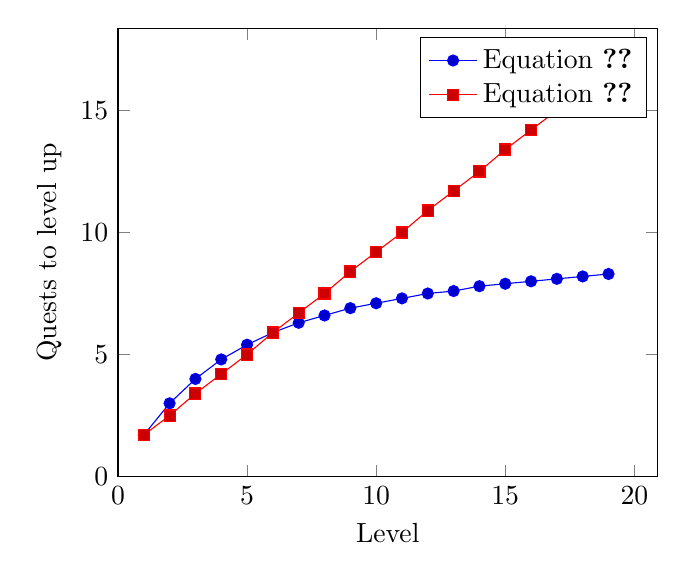
\begin{tikzpicture}
	\begin{axis}[
		xlabel=Level,
		ylabel=Quests to level up,
		xmin=0,
		ymin=0,
	]
		\addplot coordinates {
			(1, 1.7)
			(2, 3)
			(3, 4)
			(4, 4.8)
			(5, 5.4)
			(6, 5.9)
			(7, 6.3)
			(8, 6.6)
			(9, 6.9)
			(10,7.1)
			(11,7.3)
			(12,7.5)
			(13,7.6)
			(14,7.8)
			(15,7.9)
			(16,8)
			(17,8.1)
			(18,8.2)
			(19,8.3)
		};
		\addlegendentry{Equation \ref{eq:xpgainedtriangular}}
		\addplot coordinates{
			(1, 1.7)
			(2, 2.5)
			(3, 3.4)
			(4, 4.2)
			(5, 5)
			(6, 5.9)
			(7, 6.7)
			(8, 7.5)
			(9, 8.4)
			(10, 9.2)
			(11, 10)
			(12, 10.9)
			(13, 11.7)
			(14, 12.5)
			(15, 13.4)
			(16, 14.2)
			(17, 15)
			(18, 15.9)
			(19, 16.7)
		};
		\addlegendentry{Equation \ref{eq:xpgainedlinear}}
	\end{axis}
\end{tikzpicture}
\end{center}

\subsection{Gold Rewards}
\begin{equation} \label{eq:openloopreward}
	yk = ax_k + by_{k-1} + cy_{k-2}lc
\end{equation}
